\ifgerman{\chapter{Durchführung}}{\chapter{Implementation}}
\label{chap:implementation}

\section{Simulation Environment}

The FINken consists of the body, the rotors and the sensors. The body contains the behavioural and flight control, the thrust simulation is handled by scripts connected to the rotor structure.

\subsection{Scene Modeling}
\label{sec:sceneMod}

The body consists of multiple objects, while visual representation and the physical behaviour are split. 
For visual representation, a *.stl file from the CAD-Model of the original FINken was imported. 
This shape is rather complex, which makes the simulation time consuming. 
To speed up the simulation, the shape of the finken was remodelled in V-REP, using only simple rectangular shapes. 
Making the complex shape static, establishing a fixed connection and hiding the simple shape, the result is a a visual appealing simulation object with good simulation performance. 

A dummy-object is used as a singular measurement reference point in the middle of the FINken. 
This has to be taken into account when targeting physical objects, as the FINken will not be able to reach the target completely without colliding with the object. 
This dummy object should always be used when refering to the FINkens position, orientation or movements, as it is aligned to the global coordinate system while especially imported shapes may be rotated in the simulation. 

V-REP provides several pre-configured sensor type, the real FINkens sensors were modeled by using existing ultrasound distance sensors. 
The FINken is equipped with \href{http://www.maxbotix.com/documents/I2CXL-MaxSonar-EZ_Datasheet.pdf}{Maxbotix MB1232: I2CXL-MaxSonar-EZ3} sensors. 
According to the datasheet, they have an opening angle of $\ang{30}$ at maximum range when detecting smaller objects and maximum range of $2.65m$ for larger objects as walls. 
The datasheet states a rather complex beam shape, but for the simulation a cone with an opening angle of $\ang{30}$  and a height of $7.65m$ will be used, as the alternative sensor earlier had a range of $7.65m$ and in the simulation it is very easy to internally cap the values. 
Finally, a dummy target objects belongs the virtual FINken. 
This object can be moved manually in the scene and the simulated quadcopter will fly towards it.  
As the real FINken doesn't have the ability to fly to predefined points, we only used this feature for development.

\begin{figure}[h!]
 \begin{center}
  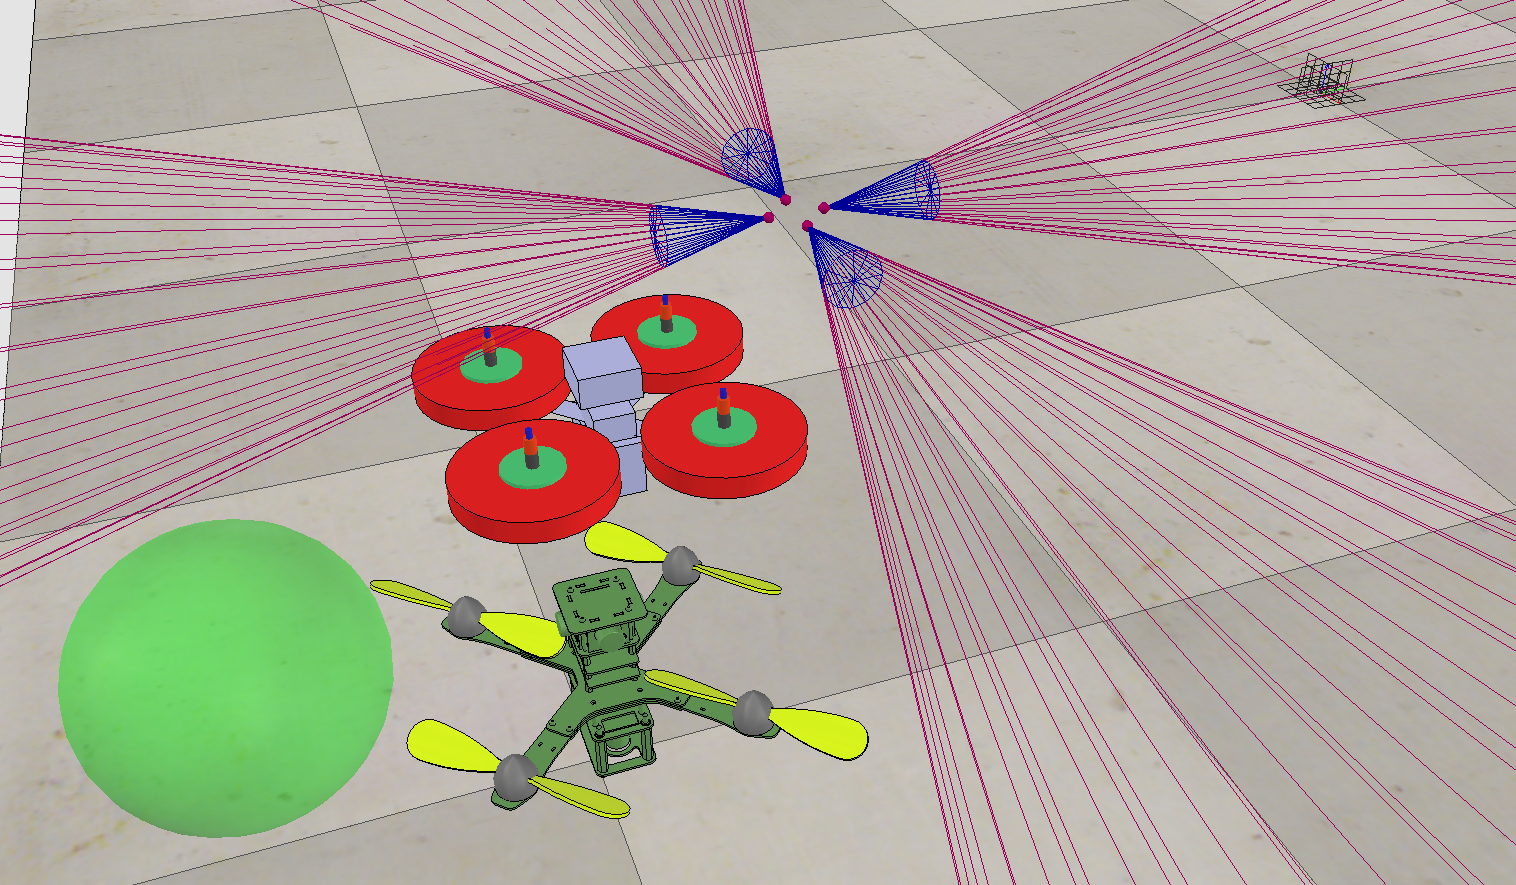
\includegraphics[width=\linewidth]{vrepDisassemlbyFull.png}
 \end{center}
  \caption{Parts of the simulation object \label{fig:vrepParts}}
\end{figure}

The measured weight of the real FINken was applied to the simulation object. 
As no advanced modelling like calculating moments of inertia was done, the weight of the motor was applied separately to the rotor model in V-REP.  The motor assembly adds significant weight outside the FINkens center of gravity and therefore has a rather large influence on its behaviour. 

\todo{check weights of real finkens}
\begin{table}[h]
	\centering
	\begin{tabular}{|l|c|c|c|}
    		\hline
		Part & Weight FINken2 & Weight FINken3 & Weight in Simulation \\
		\hline
    		Body & 178g &  214g & 284\\
    		\hline
		Motor \& rotor & 4x 15g & 4x 25 & 4x 25\\
    		\hline
		Battery & 50g & 70g & - \\
    		\hline
	\end{tabular}
    	\caption{FINken weights}
      	\label{tab:finkWeight}
\end{table}

The linear damping factor of the FINken body material was set to 0.3, to decrease drift and to model the air resistance of the real FINken, which is minimal but nevertheless existent.

\begin{table}[h]
	\centering
	\begin{tabular}{|c|c|}
    		\hline
		Parameter & Value \\
		\hline
    		Physics engine & Bullet\\
    		\hline
    		Dynamics settings & Accurate (default) \\
    		\hline
    		Simulation time step & 50 ms (default) \\
    		\hline
    		Real-time mode & enabled \\
    		\hline
	\end{tabular}
    	\caption{V-REP simulation parameters}
      	\label{tab:simSettings}
\end{table}

The rotor model in V-REP handles the thrust simulation and thus a huge part of the physical behaviour of the quadcopter model.  
Again, visual representation and physical simulation are separated. 

The visualisation is done with a static shape of a rotor, that is connected to a joint and rotates with a fixed speed. 
During flight, the rotation speed does not really change visually noticeable, a dynamic adaption of the rotation would only increase computation time without much benefit. 
Of course, the rotor shape could be made non-static and rotate in a particle stream, and apply the thrust force according to the particle collisions, but again, this would mean a massive increase of computation power and is not needed for our purposes.

\begin{figure}[h!]
 \begin{center}
  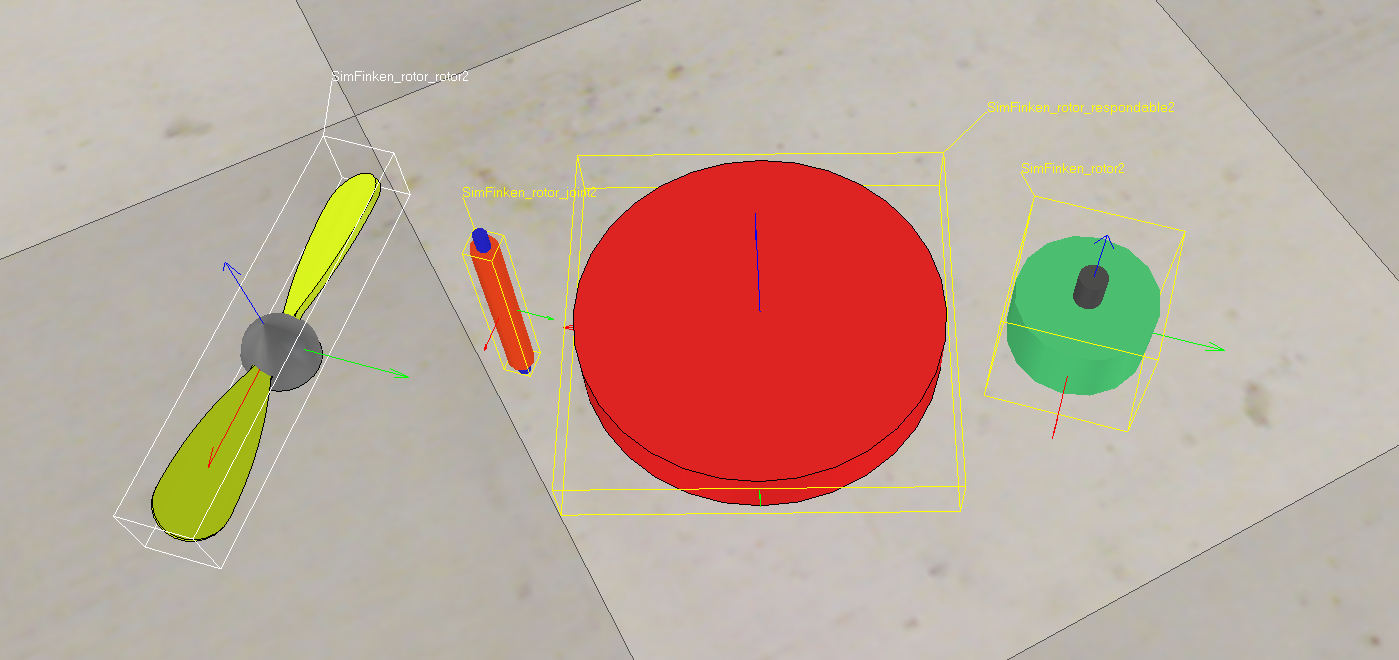
\includegraphics[width=\linewidth]{vrepRotorLegend}
 \end{center}
  \caption{Parts of the simulated rotor \label{fig:vrepRotor}}
\end{figure}


The rotor model is attached to the FINken body via a force sensor which applies the forces and torques calculated in the physical rotor model to the FINken body. 
The rotor is represented by a cylindrical shape which resembles the area swept by a real rotor and uses a particle simulation to emulate the airstream. The handling of the particle simulation is done inside a lua child script attached to the rotor model.
 
 
During simulation, the particle velocity is the parameter used to control the finken. This rotor model was already included in V-REP as an example and was used with slight  modifications, the theory behind it is shortly explained in \ref{sec:theoryRotor}. 

The particle velocity was calculated as in \ref{equ:velocity} to be $11.077 \frac{m}{s}$ under standard conditions.

 \begin{equation}
    v_{final}= 2 * \sqrt{\frac{ F_i}{2 \rho_{air} A}} = 2 \sqrt{\frac{ 0.096 kg * 9.81 \frac{m}{s}}{2 * 1.2041 \frac{kg}{m^3} * \frac{\pi}{4} * 0.1274^2 m^2}} = 11.0774 \frac{m}{s}
    \label{equ:velocity}
 \end{equation}
 
 
    
    The particle flow rate was initially set to $430 \frac{1}{s}$. 
    Our simulation step size is $50 ms$, so this would mean $21.5$ per simulation step. 
    As shown in \ref{tab:particleNum}, the maximum step size with a particle object with a capacity of $50$ particles would be $100 ms$ and simulation times below $10 ms$ might pose problems because of to few particles per step. 
   The initial flow rote thus shows a good compromise between accuracy and computation time and was further used.
    
    With a particle rate of $\dot n = 430 \frac{1}{s}$ and the final velocity $v_{final} = 11.0774 \frac{m}{s}$, the particle mass can be calculated as in \ref{equ:particleMass}
  
   \begin{equation}
    m_{px}= \frac{\dot m}{\dot n}=\frac{\frac{F_i}{2 v_{final} }}{\dot n} = \frac{\frac{0.096 kg * 9.81 \frac{m}{s}}{2 \sqrt{\frac{ 0.096 kg * 9.81 \frac{m}{s}}{2 * 1.2041 \frac{kg}{m^3} * \frac{\pi}{4} * 0.1274^2 m^2}} }}{430 \frac{1}{s}} = 1.9771 * 10^{-4} kg
    \label{equ:particleMass}
 \end{equation}
    
    Continuing with a particle diameter of $5mm$, the particle density can be obtained as in \ref{equ:particleDensity}.
  
      
   \begin{equation}
    \rho_{px}= \frac{\dot m}{\dot n V_{px}} = \frac{\frac{0.096 kg * 9.81 \frac{m}{s}}{2 \sqrt{\frac{ 0.096 kg * 9.81 \frac{m}{s}}{2 * 1.2041 \frac{kg}{m^3} * \frac{\pi}{4} * 0.1274^2 m^2}} }}{430 \frac{1}{s} \frac{pi}{6} 0.005^3 m^3} = 3020.8119 \frac{kg}{m^3}
    \label{equ:particleDensity}
 \end{equation}
    
\begin{table}[h]
	\centering
	\begin{tabular}{|c|c|}
    		\hline
		Simulation step size & Particles per step \\
		\hline
    		5 ms & 2.15\\
    		\hline
    		10 ms & 4.3  \\
    		\hline
    		25 ms  & 10.75\\
    		\hline
    		50 ms & 21.5 \\
    		\hline
		100 ms & 43 \\
    		\hline
		200 ms & 86 \\
    		\hline
	\end{tabular}
    	\caption{V-REP particles per step}
      	\label{tab:particleNum}
\end{table}


\begin{table}[h]
	\centering
	\begin{tabular}{|l|c|c|c|}
    		\hline
		Parameter & Original Value & new Value \\
		\hline
    		Particle Size & $5 mm$ &  $5 mm$\\
    		\hline
		Particle densitiy & $ 8500 \frac{kg}{m^3} $ & $3020.81 \frac{kg}{m^3} $   \\
    		\hline
		Initial velocity & $ 4 \frac{m}{s}$ & $11 \frac{m}{s}$  \\
    		\hline
		Particle count per second & $430 \frac{1}{s}$ & $430 \frac{1}{s}$ \\
    		\hline
		Maximum number of particles & $50$ & $50$ \\
    		\hline
		Particle life time & $0.5 s$ & $0.5s$ \\
    		\hline
	\end{tabular}
    	\caption{Particle simulation configuration parameters}
      	\label{tab:particleConf}
\end{table}

Using the particle simulation has the advantage of providing a  random factor that causes noise and it simulates the airstream which will influence other copters in scenarios with multiple quadcopters.

The existing rotor model in V-REP did work, but contained minor inaccuracies. The first issue was the constant particle creation rate. As shown in \ref{equ:mfr}, the mass flow rate also depends on the air velocity. Thus, the air velocity has a quadratic influence on the thrust, when only a linear one was modeled. This was corrected as in \ref{equ:pxrateNum} based on  \ref{equ:pxrate} that was derived in \ref{sec:theoryRotor}.

  \begin{equation}
    \dot n_{px} = \frac{\rho_{air} A}{2m_{px}} v_{final} = \frac{1.2041 \frac{kg}{m^3} \frac{pi}{4} 0.1274^2 m^2}{2 * 1.9771 * 10^{-4} kg} v_{final} = 38.8180 \frac{1}{m}v_{final}
    \label{equ:pxrateNum}
    \end{equation}
    
   The torque on the quadcopter was only dependant on the air velocity as well, while \ref{equ:torques} shows it's linear dependance on the thrust. Thus, a torque factor of $k_{torque} = 200$ was introduced to relate torque to thrust. 
   As the torque is applied on the rotor model, V-REP's physics engine handles the leverage of the rotor torque on the quadcopter body.





\subsection{Flight controller in simulation}

The V-REP example quadrocopter already included a position control with a subsidiary attitude control out of the box, both implemented with \gls{PID} controllers.
As the real FINken does not have an absolute position control, the control of the simulated FINken was changed to a pure attitude control.
The external input therefore was changed from a position to pitch, roll, yaw and throttle, as it is the case for the real quadcopter.
Thus, the controllers needed to be restructured and due to a different weight, the gain values had to be adjusted.
The gain values were only manually tuned. 
The FINkens reaction to different control inputs were observed and the \gls{PID} gain values were adjusted according to the behaviour.
In a nutshell, the adjusments can be summed up as follows:
\begin{itemize}
	\item{$K_P$: Increase, if the reaction is to slow, decrease if overshooting}
	\item{$K_I$: Increase to reduce steady state errors, decrease if reaction is to slow}
	\item{$K_D$: Increase if reaction to changes is to slow, decrease if overshooting for changes}
\end{itemize}

As previously mentioned in \ref{sec:sceneMod}, the virtual FINkens position and orientation is received from a dummy Object in the middle of the simulation model, comparable to the \gls{AHRS} of the real FINken.

The throttle can be directly controlled, by feeding the command signal directly to the rotors. 
Then, only a factor is applied, to get the quadcopter to hover at $50 \%$ throttle. 
However, as no feedback loop exists, the copter will drift away.
Because the real FINken does not compensate the battery voltage, the hover throttle will change during flight, making this type of control unsuitable for a mixed reality simulation.

As a solution, the height sensor of the real FINken can be used to set a target height.
Then, a \gls{PID} controller in the simulation can adjust the throttle accordingly.
For this purpose, the position controller of the original simulation with only a proportional factor was reused. 
Opposite to the real FINken, the height controller of the virtual one includes a proportional factor for the vertical speed.
\begin{equation}
thrust = 22.175 * throttle/100 +2 * e  - 2 *v_{vertical}
\end{equation}


The with only a proportional factor is symmetric, therefore the pitch and roll controller are identical.
The rotation matrix of the \gls{IMU} dummy object is compared against the target orientation.
The resulting error is forwarded to the respective instance of the \gls{PID} controller class, together with the current time step.
The \gls{PID} controller computes the correction, which is subsequently applied to the rotor according to \ref{equ:torques}.

\begin{table}[h]
	\centering
	\begin{tabular}{|l|c|c|}
    		\hline
		Parameter & Original Value & new Value \\
		\hline
    		$K_P$ & $0.25$ &  $0.2$\\
    		\hline
		$K_I$ & $0$ & $0.1$   \\
    		\hline
		$K_D$  & $2.1$ & $1.5$  \\
    		\hline
	\end{tabular}
    	\caption{\gls{PID} gain values for pitch and roll}
      	\label{tab:PIDpitchroll}
\end{table}

The yaw controller's gain parameters was estimated to the values in \ref{tab:PIDyaw}.
\begin{table}[h]
	\centering
	\begin{tabular}{|l|c|c|}
    		\hline
		Parameter & Original Value & new Value \\
		\hline
    		$K_P$ & $0.25$ &  $0.2$\\
    		\hline
		$K_I$ & $0$ & $0.1$   \\
    		\hline
		$K_D$  & $2.1$ & $1.5$  \\
    		\hline
	\end{tabular}
    	\caption{\gls{PID} gain values for yaw}
      	\label{tab:PIDyaw}
\end{table}
The original yaw controller did not take into account, that the same orientation could be described by a positive and a negative angle.
To address this issue, it has to be ensured that $-\pi<e_{yaw}<\pi$, as in the following Lua code.
\begin{center}
\begin{tabular}{c}
\begin{lstlisting}[basicstyle=\small, language={[5.2]Lua}]
	local errorYaw=euler[3]-yawTarget*(math.pi/180)
	if errorYaw < -math.pi then
		errorYaw = 2*math.pi+errorYaw
	else if errorYaw > math.pi then
			errorYaw=yawTarget*(math.pi/180)-euler[3]
		end
	end
\end{lstlisting}

\end{tabular}
\end{center}


To prevent the effect of windup of the integral part of the controller, the integral part is reset for all used controllers when the target is reached and the sign of the error changes.

\todo{position PD controller?}




\subsection{Simulation Software Structure}
\label{sec:simSoftStruct}
\tikzset{
    group/.style={
           rectangle,
           rounded corners,
           draw=black, very thick,
           minimum height=2em,
           inner sep=2pt,
           text centered,
           },
           swScript/.style={
           rectangle,
           draw=black, very thick,
           minimum height=2em,
           inner sep=2pt,
           align = left,
           },
           vrepObject/.style={
           circle,
           draw=black, very thick,
           minimum height=2em,
           inner sep=2pt,
           text centered,
           },
           vrepEnv/.style={
           ellipse,
           draw=black, very thick,
           minimum height = 5cm,
           minimum width = 3cm,
           },
            implements/.style={
            -{open triangle 60}, dashed
           },
           inherits/.style={
           -{open triangle 60},
           }
}
\begin{figure}[h]
	\centering
	\begin{tikzpicture}[scale=2, node distance = 1cm, auto]
		%vrep part
		\node[vrepEnv](vrep){};
		\node[below=0.3cm of vrep.north]{\underline{V-REP}};
		\node[vrepObject, below =1.1cm of vrep.north](fink1){finken1};
		\node[vrepObject, below =0.4cm of fink1.south](fink2){finken2};
		%lua script part
		\node[swScript, rectangle split, rectangle split,rectangle split parts=3, right=of vrep.45](finkenMeta){finkenMeta\nodepart{second}
			public:
			\nodepart{third}
			public: \\
			step() \\
			sense() };
		\node[swScript, rectangle split, rectangle split,rectangle split parts=3, below=of finkenMeta](finken){finken\nodepart{second}
			public:
			\nodepart{third}
			public: \\
			step() \\
			sense() };
		\node[swScript][rectangle split, rectangle split,rectangle split parts=3, right=of finken](finkenCore){finkenCore 
			\nodepart{second}
			public:
			\nodepart{third}
			public: \\
			step() \\
			sense()}; 
		\node[swScript, rectangle split, rectangle split,rectangle split parts=3, above=of finkenCore](finkenPID){finkenPID\nodepart{second}
			public:
			\nodepart{third}
			public: \\
			init(P,I,D) \\
			step(error, $\delta$t) };
		%connections
		\draw[inherits] (finken) to (finkenCore); 
		\draw[-{angle 60}](finkenCore) to (finkenPID);
		\draw[implements](fink1) to (finken);
		\draw[implements](fink2) to (finken) ;
		\draw[implements](vrep.45) to (finkenMeta);
	\end{tikzpicture}
	\caption{Software structure of the FINken Simulation}
	\label{fig:finkenSoftStruct}
\end{figure}

The simulation software is written in Lua and runs inside a non-threaded child script of each FINken quadrocopter in V-REP.  

The base class is the finkenCore, which contains the main flight control algorithm and a steering interface as well as an interface to the FINkens sensors.
The input commands for controlling the FINken are set via the signal communication of V-REP. Signals inside V-REP are the most versatile communication possibility which can be accessed from anywhere inside V-REP and any remote API, they can be seen as a kind of global variable. Signals can be of integer, float or string type, where custom data types can be sent in text form as string signals. 

The finkenCore needs to be initialized at simulation start the for each simulated FINken. It starts the V-REP remote API server and creates the API signals. Also, the \gls{PID} controllers for flight control are initialized. 
During simulation, calling the \textit{FINkenCore.step()} method handles the flight control. The input values are read from the signals \textit{pitch}, \textit{roll}, \textit{yaw} and \textit{throttle}. When the signal \textit{height} has a positive value, the FINkenCore will control the thrust so that the simulated FINken will keep the height provided by the signal, otherwise only the \textit{throttle} signal is used directly. The previously initialized \gls{PID} controllers are used to compute the target air stream velocity for each rotor to move the simulated FINken to the target orientation.

To keep a quadcopter at a certain height without an external reference requires an exact equilibrium between gravity and thrust. The current real FINkens do not compensate the battery voltage, so the same throttle corresponds to different thrust forces during flight. Also, each FINken unit has slightly different base thrust. Therefore, the thrust in the simulation is tuned with a logisitc curve \ref{equ:logistic} to decrease the influence of the throttle close to the hover thrust. 
\begin{equation}
	throttle_{tuned} = \begin{cases}
		-\frac{a * |throttle|}{a - |throttle| + 50} + 50 & throttle < 0 \\
		\frac{b * throttle}{b - throttle + 50} + 50 & throttle >= 0\\
	\end{cases}
\label{equ:logistic}
\end{equation}
The default values for the throttle tuning function are  $a = 1$ and $b = 1$. 
\todo{insert plot of function?}


The simulated FINken is equipped with 4 distance sensors which resemble the 4 ultrasound sensors of the real FINken. The FINkenCore module contains a \textit{sense()} function that reads the 4 distance sensors and writes the values to the signal \textit{sensor\_dist}. As signals only support limited data types, \textit{sensor\_dist} is a string signal containing a packed float array. The array contains the distances in the order \textit{front}, \textit{left}, \textit{back}, \textit{right}.  If the FINken gets more sensors in the future, their evaluation has to be added to this method.
By writing the distance values to a signal, they can be propagated to the Ivy-Bus and thus to the real FINken by our Java communication app, which enables the real FINken to detect virtual objects, as simulated FINken or walls that only exist in the Simulation.


While the FINken is normally controlled by setting the pitch, roll, yaw and throttle directly, an alternative is to specify a target object. This method was originally used by the example quadcopter model of V-REP, though the function works differently in the FINkenCore now. When calling  \textit{setTarget(targetObject)}, the differences in x, y and z coordinates of the FINken base to the target objects are given to three \gls{PID} controllers which calculate the pitch, roll and throttle to move the FINken to the target objects position. Those values are then published via the control signals for the FINken and regularly processed by it's internal controls. Therefore, \textit{setTarget(tragetObject)} needs to be called every time before \textit{step()}, when a target object should be approached.

In the previous sections, only the signal names for the first simulated FINken were used for better readability. As the simulation is scalable, more than one FINken can be added, therefore a naming scheme for signals is needed to prevent collisions of the globally visible signals. The signals corresponding to the first FINken are \textit{pitch}, \textit{roll}, \textit{yaw}, \textit{throttle}, \textit{height} and \textit{sensor\_dist}. For the second FINken, when the first one is copied, V-REP automatically adds "\#0" to it's name. Following this convention, but leaving the '\#' to prevent problems with special characters when forwarding the signals through our interface, we add '0' to the signal names for the second FINken and consecutively enumerate following FINkens.

The finken.lua module provides an basic structure for further enhancements. It's contained functions like \textit{step()} and \textit{sense()} are called called inside V-REP during the appropriate simulation step sections. By calling custom functions inside those functions, the behaviour of the FINkens can be customised without any need to change the lua scripts inside V-REP. If a heterogenous swarm of FINkens with different functionalities should be implemented, the different finken-scripts have to be imported by the different FINkens in the simulation, which needs to be done in the lua scripts inside V-REP.


FinkenMeta.lua is loaded in the child script of a dummy object in the scene  to have an API to the simulation that is not connected to a single FINken. This can be used to dynamically manipulate the environment during simulation, e.g. by adding objects like other FINkens.

\section{Communication V-REP - Quadrocopters}
\label{sec:commImplementation}

This chapter describes the implementation of the requirements on the Java-API, which ware discussed in \ref{sec:communication} of \ref{chap:theory}. It begins with an overview of the software architecture and continues with the explanation of the created projects, classes and their use. It helps understanding how the communication between the V-REP and the quadrocopters is implemented and how to use the API or extend it in order to implement other mixed-reality scenarios.\\
Note that this is just a brief explanation of the Java-API implementation. If you want to go in details refer to the Javadoc which is also provided as an attachment to this paper.

\subsection{Software architecture}

The software architecture of the Java-API, which serves as a communication bridge between the Paparazzi software and the V-REP simulation, is designed to be as modular as possible in order to facilitate the further development of the project. Its reusable components should also serve as a building blocks for the students that want to develop future mixed-reality projects. \\

On \ref{fig:apiArchitecture} is depicted an raw overview of the Java-API software architecture.
The final program is assembled from independently developed components. Each part is independent and provide well-defined exported interfaces so that the other parts can use them.
The first layer contains the projects \textit{JavaV-REP}, \textit{JavaIvyBus} and \textit{JavaXmlSax}.\\
The \textit{JavaV-REP} is the implementation of the requirements concerning V-REP, that ware discussed in \ref{sec:requirementsVREP} of \ref{chap:theory}. At the heart of this project is the V-REP Remote-API binding for Java provided by Coppelia. The \textit{JavaVrep} project extends this library and provides further utility methods for establishing connection to remote V-REP servers as well as retrieving and manipulating scene objects. The \textit{JavaV-REP} project is described in more details in \ref{sec:vrepImplementation}.\\

\begin{figure}[h!]
 \begin{center}
  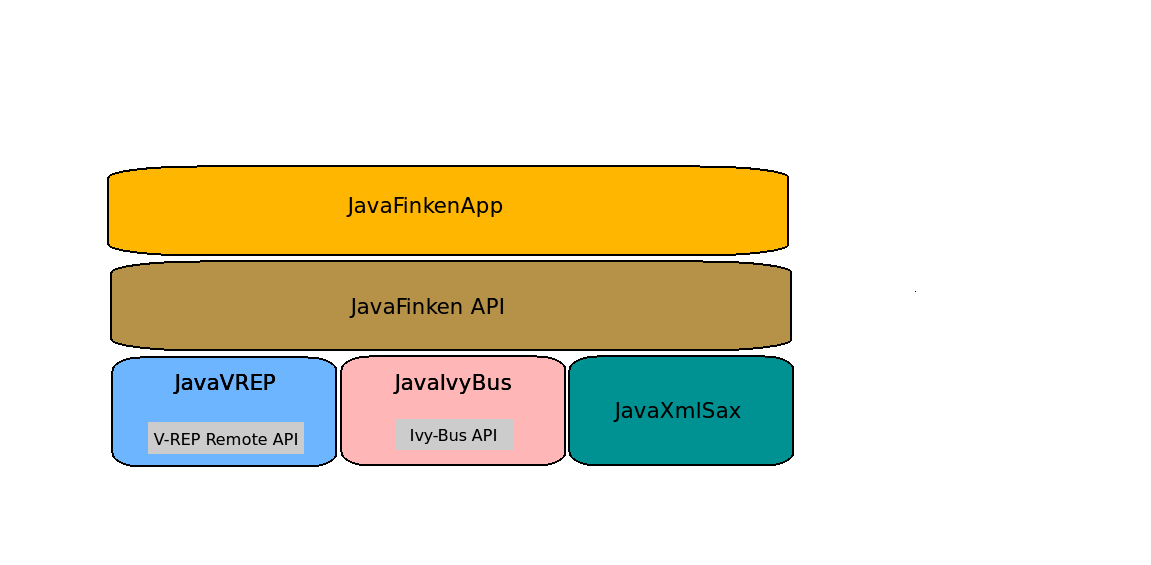
\includegraphics[scale=0.6]{apiArchitecture.png}
 \end{center}
  \caption{Java-API architecture\label{fig:apiArchitecture}}
\end{figure}

\textit{JavaIvyBus} is a Java project, that imports the Ivy-Bus library and implements the requirements regarding Ivy-Bus, which ware discussed in \ref{sec:requirementsIVYBus}.\\ 
It extends the functionality of the the Ivy-Bus library and provides the programmer with the possibility to create Ivy-Bus nodes by just instantiating an object which takes as constructor parameter the name of the bus-node. It facilitates the connection or disconnection from the bus by just calling a function the the created bus-node object. The abstractions on which this project rely also allow to easily create bus messages or just parse them from xml file and subscribe to them even dynamically. The \textit{JavaIvyBus} project is discussed in more detail in \ref{sec:ivyBusImplementation}. \\

The \textit{JavaXmlSax} project is a small API, that allows the programmer to easily create a custom xml reader that parses any xml document and retrieves the instances of the objects defined by the xml. It consists of several abstract classes, that provide the template for the custom xml readers.\\
A short explanation of how this API can be used is included in \ref{sec:xmlImplementation}. \\

On the next layer in the hierarchy is the \textit{JavaFinken} API. It uses the APIs from the layer below to provide further abstractions and utilities for our FINKEN project. It consists of classes that describe 
the aircrafts defined in the paparazzi, defines the basic classes that represent our virtual and real quadrocopters and their sensors, defines a representation of the telemetry and the V-REP signals. With the help of \textit{JavaIvyBus} API, lying on the layer below, the Ivy-Bus nodes, specific for the virtual and real quadrocopters are represented. The abstraction provided by \textit{JavaXmlSax} is used to create a custom Xml readers for parsing the telemetry, messages and aircrafts from the Xml files. A more detailed description of the API is included in \ref{sec:javaFinkenImplementation} \\

On the top of the hierarchy is situated the actual application of our project called \textit{JavaFinkenAPP}. It uses \textit{JavaFinken} API to bind the provided utility classes in a specific application meeting our project requirements. The application has a simple \gls{GUI} that facilitates specifying the IP and Port number of the V-REP simulation server, specifying path to the paparazzi software, a button for establishing the connection and other UI elements.




\subsection{Java V-REP}
\label{sec:vrepImplementation}

All the functionality, that concerns V-REP and was discussed in \ref{sec:requirementsVREP} of \ref{chap:theory} is implemented as a single Java project called \textit{JavaVREP}.\\
 The project uses the V-REP Remote-API Java binding - package \textit{coppelia} (containing 12 Java classes) and the \textit{libremoteApiJava.so} or \textit{libremoteApiJava.dll} (depending if the platform is Linux or Windows). The \textit{libremoteApiJava.so} should be placed in the Java home directory, e.g \textit{/usr/lib/jvm/java-8-oracle/jre/lib/amd64}, in order for the project to be compiled.\\
The main class is the \textit{VrepConnection.java}, which is a wrapper of the \textit{remoteApi.java} class provided by the V-REP remote API. Its singleton instance can be retrieved by calling:

\begin{center}
\begin{tabular}{c}
\begin{lstlisting}[basicstyle=\small]
VrepConnection connection = VrepConnectionUtils.getConnection();
\end{lstlisting}
\end{tabular}
\end{center}

The above expression loads the remote API library and returns the instance of \textit{VrepConnection} on which the Remote API functions are called. For example to retrieve all objects in a scene the following function have to be called on the \textit{VrepConnection} instance:

\begin{center}
\begin{tabular}{c}
\begin{lstlisting}[basicstyle=\small]

connection.simxGetObjects();

\end{lstlisting}
\end{tabular}
\end{center}

The interfaces \textit{VrepServer} and \textit{VrepClient} and their implementations \textit{StandardVrepServer} and \textit{StandardVrepClient} describe the two end-points of the communication. The \textit{VrepServer} describes the IP address and the port number of the machine on which the V-REP is running. In order to connect to a V-REP server we have to create in instance of the \textit{VrepServer} and open the client:

\begin{center}
\begin{tabular}{c}
\begin{lstlisting}[basicstyle=\small, language=Java]
VrepConnection connection;
VrepClient     client;
VrepServer     server;

connection = VrepConnectionUtils.getConnection();
client     = VrepClientUtils.getClient();
server     = new StandardVrepServer("127.0.0.1", "19999");

client.connectToServer(server);

if (!client.isConnected()) {
// error in connection
} 
\end{lstlisting}
\end{tabular}
\end{center}

The above example shows how to connect to a V-REP server. The IP \textit{127.0.0.1} specifies that the server is running on the same machine. The port number can be chosen arbitrary, but have to match on both client and server site.\\
In order to close the connection just the method \textit{client.close()} has to be called. \\

The \textit{VrepClient} conforms to the Java Beans specification and can thus fire events when the connection has been established or disconnected. Any class who is interested in catching these events asynchronously, for example \gls{GUI}, will have to implement \textit{PropertyChangeListener} and register. See
\url{https://docs.oracle.com/javase/tutorial/javabeans/writing/events.html} for more information. \\

Each V-REP scene object is represented by the interface \textit{VrepObject} and the \textit{AbsVrepObject} represents an abstract scene object from which all types of object derive. The abstract scene object has private properties like \textit{Position}, \textit{Orientation}, \textit{LinearVelocity} and \textit{AngularVelocity}, which represent its inertial parameters taken from the V-REP.
\textit{VrepObjectType} is an Enum, that specifies the scene object type like Shape, Path, Proximity sensor etc. The name of the scene object is represented by the class \textit{VrepObjectName}, which consists of a base name and an index. If an object is copy-pasted (multiple instances of an object), then
each instance of the object receives the following name, according to V-REP naming scheme: \textit{\texttt{base\_name\#index}}. For example if we want to have three quadrocopters, their names in V-REP will be represented as follows: \textit{\texttt{Quad\_Lia\_ovgu\_01}}, \textit{\texttt{Quad\_Lia\_ovgu\_02\#0}} and \textit{\texttt{Quad\_Lia\_ovgu\_03\#1}}. \\

The V-REP scene is represented by the class \textit{VrepScene}, which retrieves all objects and hold a collection of them for further use. Since we always have one V-REP scene the class is designed as a Singleton pattern. The following example shows how this class is used for loading the scene and retrieving all shape objects.

\begin{center}
\begin{tabular}{c}
\begin{lstlisting}[basicstyle=\small, language=Java]
VrepScene   scene;
List<Shape> shapeObjects;

scene = VrepSceneUtils.getVrepScene();
scene.loadScene();
shapeObjects = scene.getAllShapeObjects();

\end{lstlisting}
\end{tabular}
\end{center}

The project \textit{JavaVrep} also defines the interface \textit{ObjectUpdator} and its abstract implementation \textit{AbsObjectUpdator}, which is used to update the \textit{VrepObject}s with real-time parameters from V-REP, like their \textit{Position}, \textit{Orientation}, \textit{LinearVelocity} and \textit{AngularVelovity}.


\subsection{JavaIvyBus}
\label{sec:ivyBusImplementation}

The requirements regarding the Ivy-Bus, that ware stated in \ref{sec:requirementsIVYBus} of \ref{chap:theory} are implemented in a stand-alone Java project called \textit{JavaIvyBus}. \\
The project requires the \textit{ivy-java.jar} library to be on its class path in order to be compiled.\\
The project contains class definitions of the Paparazzi messages that are defined in a Xml file. See listing \ref{lst:MessageXml} of \ref{chap:theory}. The interface \textit{Message} and its abstract implementation \textit{AbsMessage} describe such a message with its name, period at which the message is sent, identifier and \textit{MessageField}s. \\
The interface \textit{IvyBusNode} represents a single independent node communicating on the common bus. By inheriting from its abstract implementation \textit{AbsIvyBusNode}, one can create a custom bus-node. The methods \textit{IvyBusNode.connect()} and \textit{IvyBusNode.disconnect()} are used to attach the particular node to the bus and disconnect it. The \textit{IvyBusNode} also conforms to the Java Beans specification and and fires asynchronous notifications each time the node joins or leaves the bus.
After obtaining an instance of a \textit{Message}, parsed from the Xml file or a custom-created, the bus-node can subscribe to this \textit{Message} by invoking the method \textit{IvyBusNode.subscribeToMessage(Message msg)} and thus receive all the messages of this kind or use the method \textit{IvyBusNode.subscribeToIdMessage(Message msg, int id)}, which subscribes to the messages published just by this quadrocopter ehich has the same id. \\
Once a \textit{Message} to which the bus node has subscribed has been received, the bus node fires an notification and gives the instance of the received \textit{Message}, with all of its \textit{MessageField}s initialized with the actual message values. The following listing shows an example hot to subscribe to a message and get asynchronous notification when the message is received.

\begin{center}
\begin{tabular}{c}
\begin{lstlisting}[basicstyle=\small, language=Java]

class TestBusNode implements PropertyChangeListener {
  
  private IvyBusNode node; 
  private Message    message;
  
  public TestBusNode(IvyBusNode node, Message msg) {
    this.node    = node;
    this.message = msg;
    
    this.node.addPropertyChangeListener(this);
    this.node.subscribeToMessage(this.message);
  }
  
  @override
  public void propertyChange(PropertyChangeEvent event) {
    Message receivedMessage;
    
    // the message has been received
        
    receivedMessage = (Message)event.getNewValue();    
  }

}

\end{lstlisting}
\end{tabular}
\end{center}


\subsection{JavaXmlSax}
\label{sec:xmlImplementation}

The project \textit{JavaXmlSax} was created with the idea in mind to provide a small, modular API, that gives the developer an abstract building block for fast and easy development of custom XML file readers. It uses the \href{http://www.saxproject.org/}{SAX Java API} and extends it in order to provide a template for fast creation of specific XML readers.\\
The basic class in this module is the abstract class \textit{AbsSaxXmlReader}. It encapsulates all necessary classes needed for creating and handling of the XML parsing and defines abstract methods, which allow its subclasses to provide their specific parsing criteria. Thus the developer can concentrate on the actual parsing logic and don't have to take care of setting up and managing the necessary input streams and files.\

To create a specific XML reader we have to create a class, which extends the \textit{AbsXmlReader} and provides implementation of the abstract methods \textit{onStartElementRead} and \textit{onStopElementRead}.These methods are called when the \textit{AbsSaxXmlReader} encounters start or end XML tag. It is the role of the subclass to fetch the necessary attributes and create an instance of the XML element, when \textit{onStartElementRead} is called and store the instance in some sort of collection, when the closing tag of the element is reached. In order to start the parsing process the method \textit{parseXmlDocument} of the parent class \textit{AbsSaxXmlReader} has to be invoked. \
A XML parser reads the whole XML file and returns the instances of all elements. In some case not all elements may be required and to save time and memory it would be preferred to stop the parsing after an element of interest has been found. Since the original Java SAX API does not provide the possibility to stop the parser after it has been started, we have implemented an mechanism for this.
In order to stop the parsing, the method \textit{stopParsing()} has to be invoked. The function throws a custom defined Exception - \textit{StopParsingException}, that is handled in such a way, that the method \textit{parseXmlDocument()} returns immediately.

The code below shows an example of how the XML parser can be used.

\begin{center}
\begin{tabular}{c}
\begin{lstlisting}[basicstyle=\small, language=Java]

MessageXmlReader msgReader;
List<Message>    messages;

msgReader = new MessageXmlReader("/home/paparazzi/conf/messages.xml");

msgReader.parseXmlDocument();

messages  = msgReader.getMessages();

\end{lstlisting}
\end{tabular}
\end{center}

\

The \textit{MessageXmlReader} is a class that extends the \textit{AbsXmlSaxReader} and provides implementation of its abstract methods. It returns all instances of messages contained in the \textit{/home/paparazzi/conf/messages.xml} file. The need to retrieve all messages was discussed 
in \ref{par:messageRetrieval}. \

The \textit{MessageXmlReader} gives us a significant flexibility. Since it returns a list containing the instances of all messages, we can choose a messages of interest and subscribe/unsubscribe even dynamically at run-time to them. This can be extremely useful if some quadrocopter needs some message just for a limited time, for example calibration messages, and then needs to unsubscribe from this message. Subscribing to less messages on the \hyperref[sec:ivyBusImplementation]{Ivy-Bus} can save computation time. \

Another example of XML reader, that extends the \textit{AbsXmlSaxReader} is the \textit{AircraftXmlReader} class. It is used to retrieve all aircrafts and its parameters from the 
\textit{/paparazzi/conf/conf.xml} file and has been discussed in \ref{par:aircraftRetrieval}. 


\subsection{JavaFinken}
\label{sec:javaFinkenImplementation}

The \textit{JavaFinken} API is a project that relies on the previously introduced projects \textit{JavaV-REP}, \textit{JavaIvyBus} and \textit{JavaXmlSax}. It represents the implementation of the application requirements introduced in \ref{sec:requirementsApplication} and provides the basic classes and utilities upon which our application can be built.\\

The class of a special importance is the \textit{AbsFinkenDrone}, which represents the abstract quadrocopter and is described by the interface \textit{FinkenDrone}, which on itself extends the \textit{VrepObject} interface.\\
The virtual and real quadrocopters are represented by the classes \textit{StandardRealFinkenDrone} and \textit{StandardVirtualFinkenDrone}, which extend the abstract \textit{AbsFinkenDrone}.\\
The class \textit{FinkenDroneScanner} is used to retrieve the instances of the quadrocopters and can be used as follows:

\begin{center}
\begin{tabular}{c}
\begin{lstlisting}[basicstyle=\small, language=Java]

List<StandardRealFinkenDrone>    realDrones;
List<StandardVirtualFinkenDrone> virtualDrones;
FinkenDroneScanner               droneScanner;

droneScanner  = new FinkenDroneScanner();
realDrones    = droneScanner.retrieveRealDrones(this.scene, this.client);
virtualDrones = droneScanner.retrieveVirtualDrones(this.scene, this.client);

\end{lstlisting}
\end{tabular}
\end{center}

\subsection{JavaFinken App}
\label{sec:javaFinkenApp}

The final application, that has been created upon the described above modules: \hyperref[sec:vrepImplementation]{Java-VREP}, \hyperref[sec:ivyBusImplementation]{JavaIvyBus}, \hyperref[sec:xmlImplementation]{JavaXmlSax} and \hyperref[sec:javaFinkenImplementation]{JavaFinken}  is the \textit{JavaFinkenApp}. The application has a small \gls{GUI}, that allows to specify an IP address and Port number of the machine, where the V-REP simulation is executed and also the IP address of the PC, where the Paparazzi ground station is running. This allows to distribute the Simulation on different machines like shown in \ref{fig:communication}.
By default the the local machine IP Address \textit{"1.0.0.127"} is chosen. 

\begin{figure}[h!]
 \begin{center}
  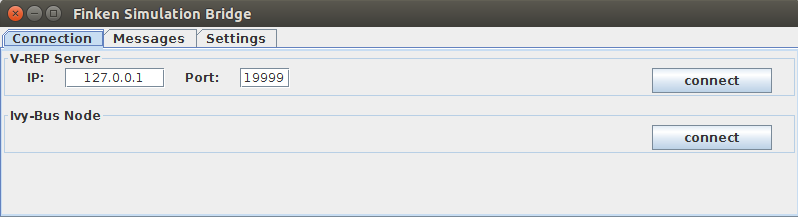
\includegraphics[scale=0.7]{FinkenSimulationBridge_GUI_1.png}
 \end{center}
  \caption{FinkenSimulationBridge \gls{GUI} connection panel\label{fig:finkenGUI1}}
\end{figure}

On the above figure \ref{fig:finkenGUI1} you can see the connection panel of the \gls{GUI}, where the IP addresses have to be specified. The path to the \textit{conf.xml} file, which stores the aircrafts and the path to the telemetry file have to be specified. The \gls{GUI} provides separate tab for this. See figure \ref{fig:finkenGUI2}.

\begin{figure}[h!]
 \begin{center}
  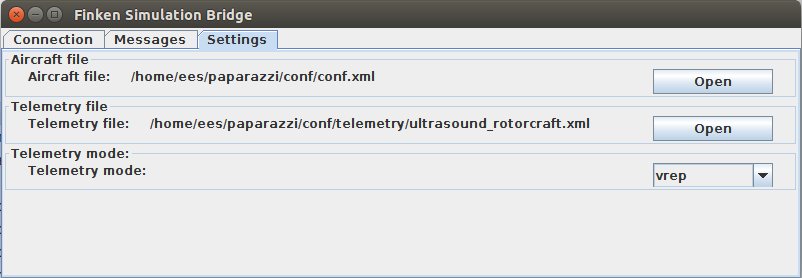
\includegraphics[scale=0.7]{FinkenSimBridge_GUI_2.png}
 \end{center}
  \caption{FinkenSimulationBridge \gls{GUI} telemetry panel\label{fig:finkenGUI2}}
\end{figure}

After choosing the path to the telemetry file, the telemetry modes are parsed from this file and are  provided for choosing in the combo-box of the \textit{Telemetry mode} sub-frame. Thus a custom telemetry mode, defining the messages that the quadrocopter needs to subscribe to, can be chosen. \\

The \href{http://www.oracle.com/technetwork/articles/javase/index-142890.html}{Model-View-Controller} (MVC) design has been used to implement the \textit{JavaFinkenApp}. The main class is the \textit{FinkenSimBridge}, which contains the main method, where the program starts. The \textit{FinkenSimBridgeView} defines the View - \gls{GUI} components. And the \textit{FinkenSimBridgeController} plays the controller role. \\

In order to start the communication, the "connect" button has to be clicked. The V-REP simulation must had been started in order to establish a connection. The listing below shows the method, executed by pressing the connect button.

\begin{center}
\begin{tabular}{c}
\begin{lstlisting}[basicstyle=\small, language=Java]

void onConnect(VrepServer _server) {

  this.vrepClient.connectToServer(_server);

  if (this.vrepScene.isLoaded()) {
    return;
  }

  this.vrepScene.loadScene();

  this._retrieveVirtualDrones();

  this._retrieveRealDrones();

  this._initVirtualDrones();
  this._initRealDrones();

}
        
\end{lstlisting}
\end{tabular}
\end{center}

The function is triggered when the connect button is clicked and takes as input argument the \textit{VrepServer}, which contains the IP Address and port number of the V-REP simulation. Then the \textit{VrepScene} is loaded and all V-REP objects are retrieved. After the scene is loaded, the virtual and real drones are fetched from the scene and stored in a list structure. The function \textit{initRealDrones()} makes the final initialization of the drones.

\begin{center}
\begin{tabular}{c}
\begin{lstlisting}[basicstyle=\small, language=Java]

  private void _initRealDrones() {
    for (RealFinkenDrone drone : this.realDrones) {
      drone.joinIvyBus();
      drone.loadTelemetryData(new File(TELEMETRY_FILE));
      drone.startPublish();
    }
  }

\end{lstlisting}
\end{tabular}
\end{center}

First the drone is attached to the Ivy-Bus, then the telemetry data is loaded and the drone subscribes to the messages that reside in the specified telemetry-mode of the telemetry XML file. Eventually the the real drones start to get updated with the proximity-sensor data and to publish it as a message on the Ivy-Bus. The function \textit{initVirtualDrones()} does the same initialization for all the virtual drones retrieved from the V-REP scene.



\section{Quadcopter}
\label{sec:finken}
This project was about to build a mixed reality simulation around the FINken quadcopter, so there weren't made many changes to the quadcopter and the firmware itself. A few changes were needed, regarding calibration, the message link and the communication from V-REP to the FINken. At the start of the project, the FINken II was used, but when the FINken III was released, it could directly be used as all our needed functions were compatible. In fact, the new telemetry link of the FINken III made a much faster communication possible, which helped some delay issues with V-REP as put in \ref{sec:messLink}
\subsection{FINken calibration}

The pitch, yaw and roll angles of the quadrocopter are measured from the Inertial-Measurement-Unit (IMU). The IMU sensor may not be mounted perfectly level to the airframe due to construction issues, imperfect soldering of the sensor on the board or just a factory defect. Such issues will cause a big offset in the sensor readings and will be critical for our simulation.
This was the case with the very first experiments. The quadrocopter in the V-REP simulation started to drift heavily from the real one at the very beginning of the simulation. As a result the quadrocopter was flying away from the simulated arena, although the real one was flying stable in the physical arena.\\
Fortunately, the Paparazzi project already provides a \href{http://wiki.paparazziuav.org/wiki/ImuCalibration}{IMU calibration software}, which we used to calibrate the accelerometer. The calibration is implemented as a python script, that has to be run on the log file containing the accelerometer calibration data. The calibration procedure was easy to perform and we had to follow the following procedure:

\begin{itemize}
\item{Flash the board with our firmware}
\item{Switch to the "raw sensors" telemetry mode via GCS->Settings->Telemetry and launch "server" to record a log}
\item{Move the IMU into different positions to record relevant measurements for each axis. }
\item{Stop the server so it will write the log file}
\item{Run the Python script on it to get the calibration coefficients and add them to the airframe file}
\end{itemize}


The listing below shows our airframe file - \textit{/paparazzi/conf/airframes/ovgu/6imucalib.xml} with the calibration coefficients resulting from the calibration.

\begin{center}
\begin{tabular}{c}
\begin{lstlisting}[basicstyle=\small, language=XML]

 <section name="IMU" prefix="IMU_">
   ...
   <define name="ACCEL_X_NEUTRAL" value="10"/>
   <define name="ACCEL_Y_NEUTRAL" value="12"/>
   <define name="ACCEL_Z_NEUTRAL" value="34"/>
   <define name="ACCEL_X_SENS" value="4.86375969658" integer="16"/>
   <define name="ACCEL_Y_SENS" value="4.86831208708" integer="16"/>
   <define name="ACCEL_Z_SENS" value="4.90201085317" integer="16"/>
   ...
 </section>
        
\end{lstlisting}
\end{tabular}
\end{center}

When a new firmware is flashed to the quadrocopter, the paparazzi software also flashes the calibration coefficients from the airframe file so that IMU gets calibrated. \\
We observed a big improvements in the simulation performance after calibrating the IMU. Although the quadrocopter was still drifting to some extend, the strong drifts have disappeared. \\
The calibration software also provides calibration for the gyroscope sensor. Although the drift in the gyro sensor is also very critical for the simulation performance, we did not perform any calibration on the gyroscope. The reason was, that the calibration of the gyroscope is very sophisticated and required a moving platform for each sensor axis, which was not present at the time of the project. However we believe, that calibration of the gyroscope will improve the results to a significant extend and should be performed in the future work of the project.


\subsection{FINken message link}
\label{sec:messLink}
In the beginning of this project, the second iteration of the FINken, the FINken II was used. 
There, the telemetry link was implemented with Bluetooth LE.
It showed, that the data rate was barely sufficient when the quadcopter was next to the computer running the ground station and dropped heavily with more distance.
The simulation runs with a time step of $50ms$, so it is desirable to get the telemetry message at the same rate to provide new data for each simulation step.
This was not possible with the bluetooth link.

The FINken III that was introduced during this project features 802.15.4 based communication.
This evolution has two major benefits.
First, in allows to send telemetry data with every $21ms$, even multiple messages, so it could be ensured that at least on average, a new message would be available for each simulation time step, even if one package is dropped.
Second, in the new communication, the quadcopter broadcasts it's data.
This allows to have multiple quadcopter connected to the same groundstation and the groundstation receives data as soon as the FINken is switched on.
The latter is a valuable improvement over the necessary linking for the bluetooth communication of the FINken II.



\subsection{V-REP to FINken communication}
The focus of the project lied on the communication from the real hardware to the simulation.
However,to make virtual objects visible to the real FINken, they need to be send somehow from the virtual scene to the real world.
The FINken relies on the ultrasound sensors to detect object, therefore especially the virtual distances to objects needs to be transmitted.
Paparazzi provides a two way communication with the telemetry link.
Thereby the existing solutions could be used to send the messages, as we as well implemented the communication structure bidirectional.

The modules of the FINken's firmware can subscribe to telemetry messages.
Since the ultrasound sensors are handled in one module, it is easy to include a subscription to our virtual distance data into the module.
At the moment, the distance sensor are only used for collision avoidance, so only the closer object is interesting.
Therefore, the integration of the virtual values was done by using the minimum value of the real and virtual distance measurements.
This ensures, that the real FINken will try to avoid any detected object, be it detected by its own sensors or by the sensors of its virtual counterpart.



